\chapter{Outlooks and conlusion}
\chaptermark{Outlooks and conlusion}
\cleardoublepage

\minitoc
\section{Introduction}
\begin{refsection}
  In this manuscript I presented a large part of the work done on the study, design and testing of non-invasive profilers based on ionization. This chapter describes the tasks currently underway or in perspective for the conception of the final diagnostics and summarize the previous chapters. 

  \section{Final design and outlooks}
  The following sections present current actions for the design of the final detectors as well as the more distant perspectives. The type of these tasks is quite broad, so it is interesting to describe them briefly.

  \subsection{Improved IPM design}
  During the tests done at IPHI, we used a simple CF200 flange to support the IPM (Fig. \ref{chap4:IPM_photo2}). For the manufacturing of the IPM, we thought that two independent flanges CF200 and CF160 (Fig. \ref{chap5:fig:bride_double}) will ease the assembling process and also the maintenance. This later configuration presents the following advantages.

  \begin{figure}[!ht]
	\begin{subfigure}[t]{0.25\textwidth}
		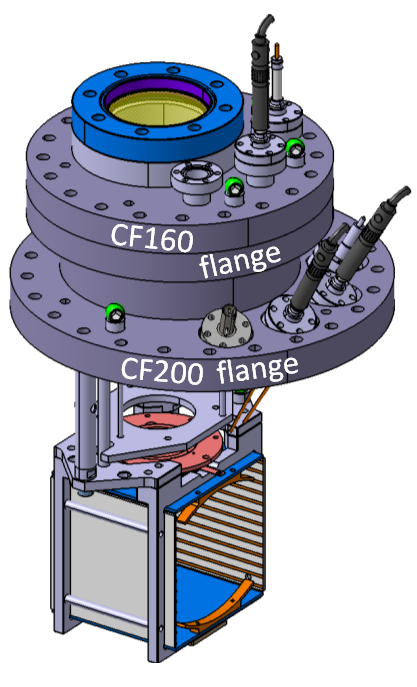
\includegraphics[width=\textwidth]{05_Conclusion/figures/fig000_bride_double2_a}
		\caption{A 3D drawing of the new design.}
		\label{}
	\end{subfigure}
	~
	\begin{subfigure}[t]{0.75\textwidth}
		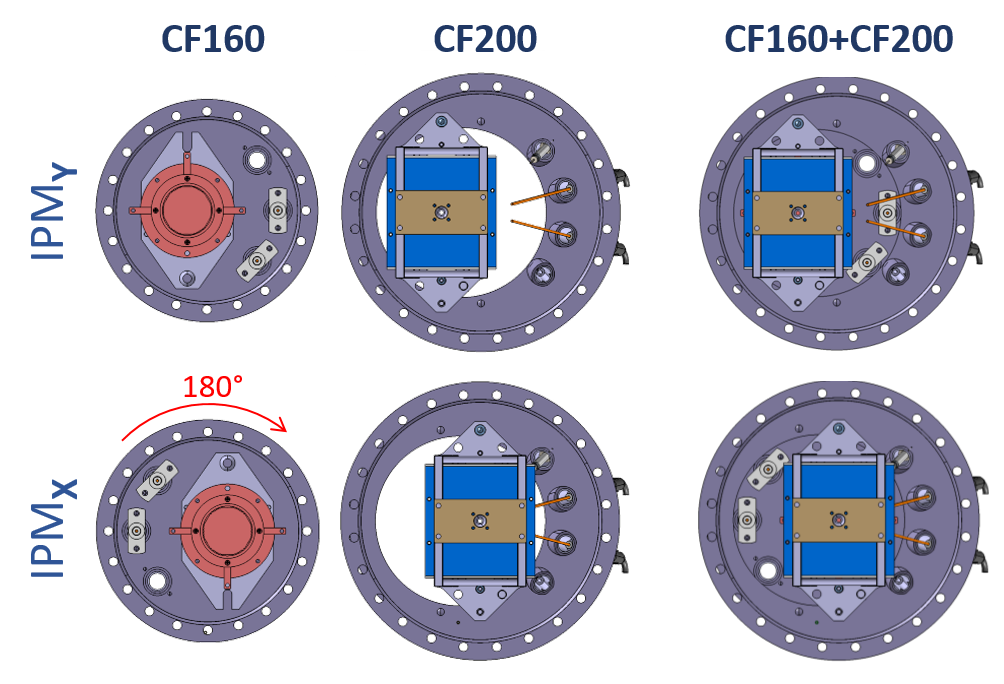
\includegraphics[width=\textwidth]{05_Conclusion/figures/fig000_bride_double2_b}
		\caption{The new design allow to remove MCP easily and is independent to the IPM direction.}
		\label{}
	\end{subfigure}
	\caption[The new IPM design]{The new IPM design \cite{JacquesCDR2019}.}
	\label{chap5:fig:bride_double}
\end{figure}

  Once the complete IPM set is mounted on the LWU, alignment can be done by measuring all sight pods on the CF200. Then, if MCP has to be removed (unscrew the CF160), the IPM cage linked to the CF200 stays fixed. MCP can be changed but, no alignment are necessary. We just have to measure with the CMOS camera the four crosses which will be engraved on the electrode plate back. This new configuration is compliant with a better reliability of the IPM since the MCP change may be done quickly, with no impact on alignment. Furthermore, the CF160 flange with its MCP bracket, HV viewports is quite light and can be easily operated.

  For assembling the whole IPM, it is more convenient to prepare first the CF200 and all its belonging items, and then the CF160 ones. It allows minimizing the MCP in oxygen atmosphere. Furthermore, the set made of CF160 and MCP holder is light with a small lever arm easy to manipulate.

  The IPMs X and Y are similar: while X is centered on the CF200 LWU viewport, Y is shifted by $36\,\mathrm{mm}$ to its CF200 axis. The trick for mounting both IPMs, is to rotate the CF160 by $180°$ wrt the CF200 flange. This is of great interest for manufacturing purpose.

  \subsection{MCP calibration}

  \begin{wrapfigure}{l}{0.5\textwidth}
  \includegraphics[width=0.5\textwidth]{example-image-a}
	\caption[The calibration of the MCP is done with a VUV lamp]{The calibration of the MCP is done with a VUV lamp.}
	\label{chap5:fig:UV_calib}
\end{wrapfigure}

  MCPs are mandatory to measure a profile with IPM in the ESS conditions. Unfortunately, these devices are sensitive to ageing effects. The gain will decrease over the time in the areas impacted by ions. Since the ESS beam may not move so much the middle area of the MCPs will be more affected. Therefore, at some point the profile measurement will be no longer correct. To overcome this phenomenon it is necessary to calibrate MCP regularly, i.e. perform a gain mapping and rectify the profile. This requires a uniform and stable source that regularly irradiates the MCP. The most common method relies a VUV source. MCPs become sensitive to the photoelectric effect for wavelengths shorter than $200\,\mathrm{nm}$. The most basic VUV sources are deuterium discharge lamps that have broadband emission with a peaks at $160\,\mathrm{nm}$. It is also possible to generate VUV with excimer lasers or by using high order harmonic generation. Thermoionic emission was discarded due to the requirements imposed by the superconducting cavities. We are also considering the use of Electron Generator Arrays. The calibration is currently being tested on the IPM test bench and Fig. \ref{chap5:fig:UV_calib} shows the principle of the experiment.

  \subsection{Remote acquisition system}
  In the case where the radiation background should shorten the MCP lifetime down to a year, it would be necessary to set a camera at remote distance in a shielded area. Two solutions are investigated to transport the image over up to $10\,\mathrm{m}$, where the camera can be shielded in the bottom of the nearby Stub. The solution to get a camera detecting single events, i.e. an ion hitting the MCP is been studied at ESS. The document presents two alternative imaging systems: the first one using a fiberscope and lenses is sketched on Fig. \ref{chap5:fig:schematic:1}, while the other one based on 2 mirrors and an objective lens can be seen on Fig. \ref{chap5:fig:schematic:2}.

  \begin{figure}[!ht]
	\begin{subfigure}[t]{0.5\textwidth}
		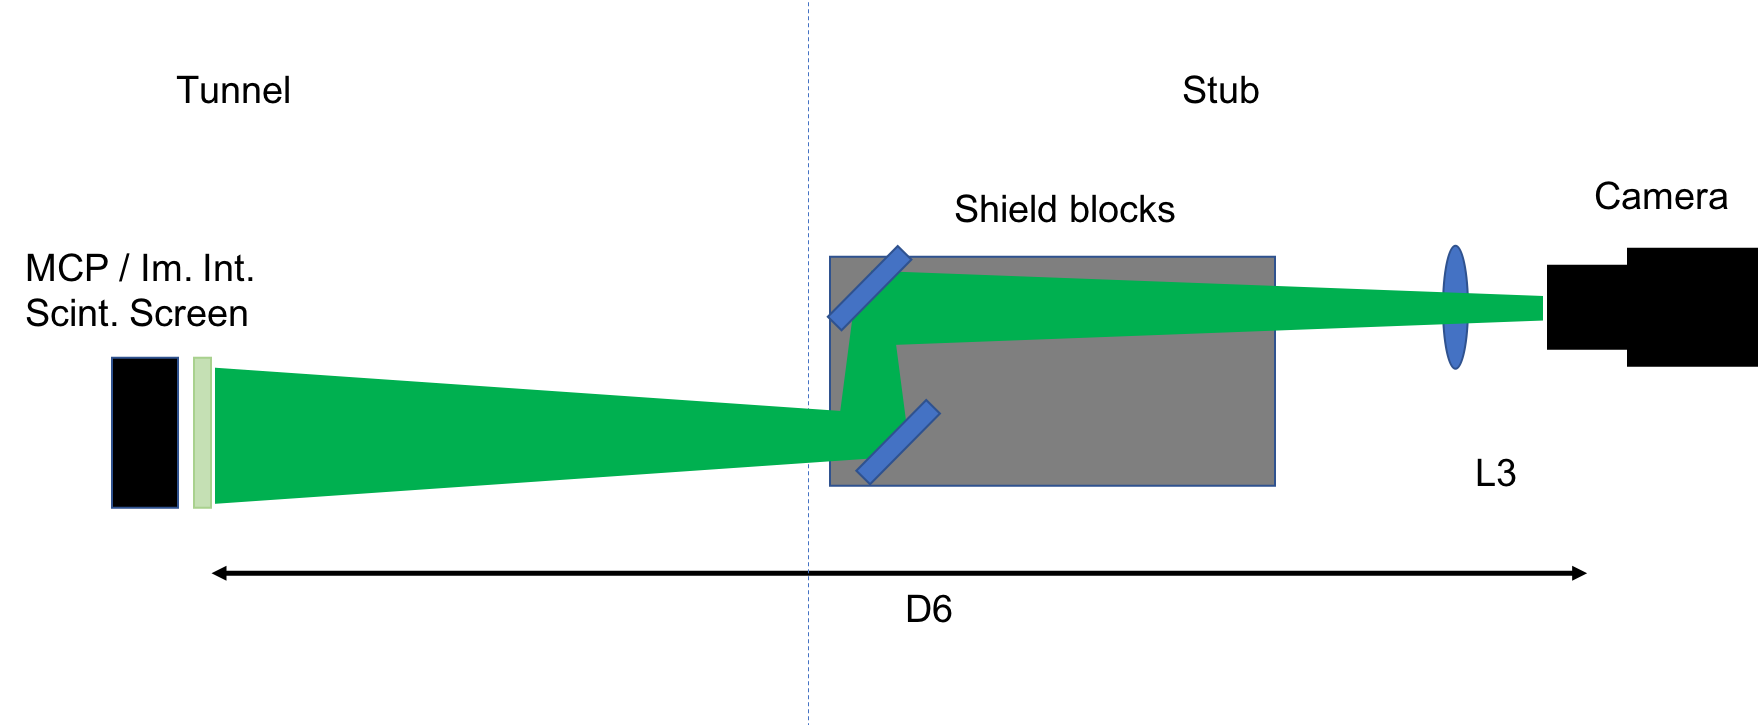
\includegraphics[width=\textwidth]{05_Conclusion/figures/fig000_schematic_telescop_lens}
		\caption{}
		\label{}
	\end{subfigure}
	~
	\begin{subfigure}[t]{0.5\textwidth}
		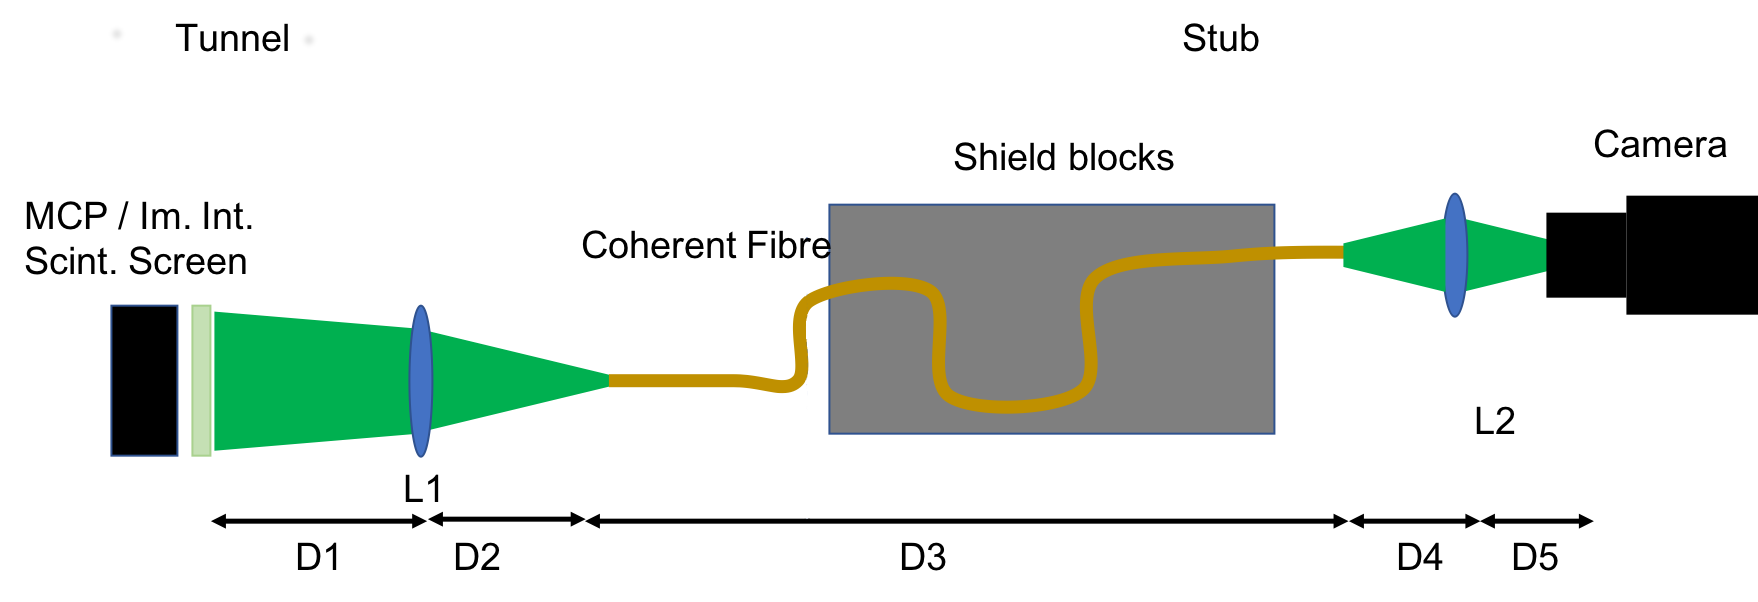
\includegraphics[width=\textwidth]{05_Conclusion/figures/fig000_schematic_coherentr_fiber}
		\caption{}
		\label{}
	\end{subfigure}
	\caption[]{}
	\label{chap5:schematic}
\end{figure}


  At a first order evaluation of the system transmission, one can start by selecting the focal lens required to make conjugate images. For the lens L1, the magnifications for the MCP is set, so as the geometrical aperture coupling light into the fibre.

  % The MCP is 40\,mm diameter and the fiber diameter is 2\,mm. The geometrical transmission T of the lens to the fiber is defined by the aperture of the lens, called the F-number or F\#, the focal lens, F and the distance between the screen and the lens, D1:
  % \begin{equation}
  %   T=\frac{1}{2} \left(1 - cos\left(\theta\right)\right)
  % \end{equation}
  % with $\theta = \rm arctan\left (\frac{F/F\#}{2D}  \right )$

  The geometrical transmission for 0.5 numerical aperture of the fiberscope is about $3 \cdot 10^{-5}$ while it is a factor 4 below for the second system. Such an attenuation encourages to purchase stacked double MCP for increasing the output light.

  The fiber attenuation is an important value to take into account. For instance, for silica fibers, this can be as low as a few $\mathrm{dB/km}$. We intent to used plastic coherent fibers. The material used is PMMA. This material is rather cheap, and it presents good optical quality and rather good transmission, typically $0.5\,\mathrm{dB/m}$ at $500\,\mathrm{nm}$. However, a full characterisation of the system with the selected fiber will have to be done in order to prove and demonstrate the performance of the system. Lenses transmissions can be close to $100\,\mathrm{\%}$ with anti-reflection coating.

  \subsection{Background signal estimation}
  During the project reviews we were asked to study the influence of background noise on the IPM readouts. This is a complex task because it requires sufficient information on the particles involved in background noise and realistic geometry. Without these two conditions the results may not be relevant

  \begin{wrapfigure}{r}{0.5\textwidth}
  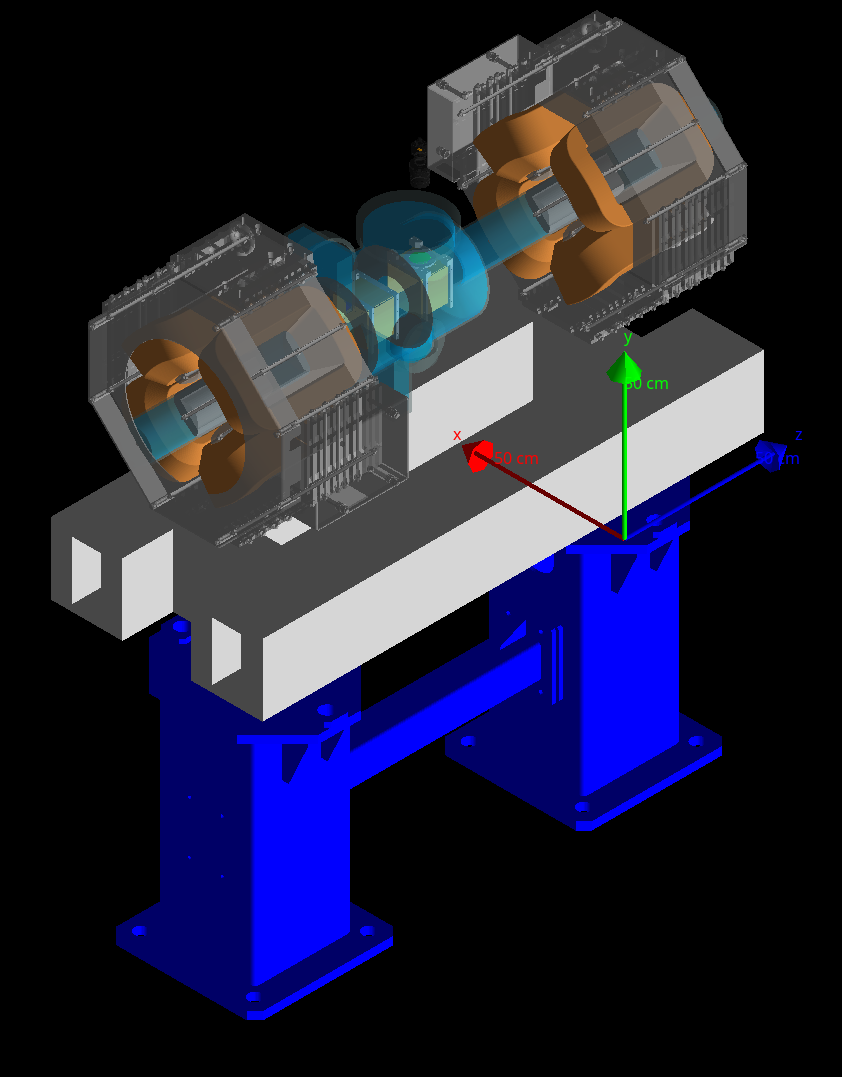
\includegraphics[width=0.5\textwidth]{05_Conclusion/figures/fig000_geant4_sim}
	\caption[The geometry implemented in Geant4]{The geometry implemented in Geant4.}
	\label{chap5:fig:Geant4}
\end{wrapfigure}

  During the thesis, a Geant4 simulation was started in order to answer this request. The simulation includes a mixed geometry including shapes made from primitive geometry (LWU, support, MCP) and complex elements imported from CAD files (IPM, camera, magnet). The Fig. \ref{chap5:fig:Geant4} shows the implemented geometry of the LWU with the two IPMs, the quadrupoles and the cameras with their sensors. The choice of the physics list can be quickly modified using the predefined lists in Geant4. The elements to be studied use the Sensitive Detector mechanism enabling to save information about the particles passing through them. As data flow is important, the simulation results are saved using the ROOT interface provided in Geant4. The simulation uses the new multithreading features of latest versions of Geant4 and an OpenMPI layer has been added.

  Unfortunately, the information about the background particles was finally given after the beginning of the writing phase of this thesis. Nevertheless, the simulation base is implemented and I hope that this work will continue and lead to results that may provide additional knowledge.

  \section{Overview of the thesis}
  %In this thesis I participated in the simulation, design and testing of ionization profile monitors prototypes for the proton linac of the European Spallation Source.

  \subsection{The ESS linac and IPM}
  Intense neutron sources are very difficult to achieve. Historically, nuclear reactors have been widely used as intense neutron sources. In Europe the situation is quite critical because most of research reactors will close within the next decade. In that context, the European Spallation Source is being built close to Lund, in Sweden. ESS will push back the limits of existing spallation sources by means of an high end powerful linear accelerator. To ensure the safety of the machine during the commissioning and operations, many diagnostics are foreseen along the accelerator. 
  
  This thesis described the design of one of these diagnostics: the Ionization Profile Monitor(IPM). IPMs are based on the ionization of residual gas. This is one of the most effective methods, but it is nevertheless quite complex to implement. The first IPMs date back to the 1960s but the method has been improved significantly with advances in detector, electronics and computer sciences.The IPM method is now mature and used in several installations. In this thesis, the existing methods have been reviewed in order to find the best solution that may match with the ESS requirement. This have been done by simulations first and, in a second time, by building and testing prototypes.

  \subsection{IPM feasibility}
  Three key points had been identified: number of primary particles, distortion effects of the profile, the choice of the reading system.

  The conditions at ESS are particularly unfavorable for the ionization cross sections and the high vacuum in the accelerator does not work in our favour. Calculations (Bethe and PAI) and simulations show that the order of magnitude of the number of primary particles is about a few thousand particles per pulse beam under nominal ESS conditions. This number seems sufficient to carry out a measurement assuming that tey are correctly detected.

  Non-uniformities of the electric field can be effectively corrected using field correctors and separation discs regardless of the power supply configuration used. However, the symmetrical mode is easier to correct and reduces the maximum voltage level required.
  Simulations clearly show that ions are less sensitive to the space charge effect and initial velocity of particle. Measurement with electrons introduces an error that does not allow the ESS requirements to be met. It is impossible to install a corrector magnet to constrain the electron trajectories. Therefore, the profile measurement will be done with ions.

  The use of ions makes the choice of the readout a more complicated. Strips are an robust method but require enough sensitive and low-noise electronics to be able to detect such low charge quantities.
  The MCPs amplifies the signal but these devices tend to age. Silicon detectors look very promising because they are very sensitive, resistant and fast. However, the detection of low energetic ions is not ensured and the implementation is quite complex.

  \subsection{Prototype design and tests}
  First, the feasibility of silicon detectors was verified on the
  At IRMA ion implanter, the feasibility of silicon detectors was checked. 
  The detection seams possible but with almost no error margin. We also observed that the silicon sensor was quickly damaged by the incident ions. Therefore, we discarded this readout for ESS usage.
  
  Then, a complete IPM testing platform has been developed in order to test the two remaining readouts. The IPM prototypes have been designed to be totally independent to the readout. Therefore the testing platform was quite versatile. 

  The prototype been tested at IPHI, a $3\,\mathrm{MeV}$ proton accelerator. A complete characterization of the two IPMs was done.Good agreements have been found between the two types of IPMs and existing IPHI diagnostic. The tests were also a kind a commissioning of the machine confirming that the IPMs is a great tool to tune a beam. According to results the measurement seams possible at ESS with even a single stage MCP. The results has been presented to ESS collaborators during a Critical Design Review.

  The final IPM will use double stages MCP polarized in symmetric HV configuration. The symmetric setup provides really good uniformity with basic corrections. It also reduces the maximum potential to apply to electrode. 
  A MCP with strips may provides best performances in term of sensitivity and speed. But a complicated reading electronic must be designed for that purpose. Whereas a MCP optical exposes decent performances and an high resolution but the acquisition relies only on COTS cameras.
  At the end the optical solution was chosen. Anyway the design of IPMs allows to easily upgrade the readout for future improvements.
  
  The double stage MCP will allow measurement during the accelerator commissioning. Therefore may be ready even before than the accelerator reaches its nominal conditions. On the other hand the use of an double stage MCP reduces the maximal resolution but this reduction is less important compare to the one induced by the remote acquisition system

  The final IPMs will be produced following the ESS requirement for the superconducting cavities. This means that the IPMs will be assembled within an ISO-5 clean room environnement. The IPMs will be delivered by pair and the first pairs is expected to be delivered to ESS in the beginning of 2020.

  %\subsection{Personal conclusion}

\end{refsection}